% This is samplepaper.tex, a sample chapter demonstrating the
% LLNCS macro package for Springer Computer Science proceedings;
% Version 2.20 of 2017/10/04
%
\documentclass[runningheads]{llncs}

\usepackage{graphicx}   % Images
\usepackage{tabularx}   % Tables
\newcolumntype{C}{>{\centering\arraybackslash}X} % Table uses all width and it's centered
\usepackage{hyperref}
\hypersetup{
    colorlinks = true,
    linkcolor = blue,
    filecolor = blue,
    citecolor = black,      
    urlcolor = black,
}

% If you use the hyperref package, please uncomment the following line
% to display URLs in blue roman font according to Springer's eBook style:
% \renewcommand\UrlFont{\color{blue}\rmfamily}

\begin{document}
% Title
\title{Solver of Tricky Triple Puzzles Based on Constraint Programming}
% Abbreviated Title
\titlerunning{Tricky Triple Solver}

% Authors
\author{
    \begin{tabular}{l r}
        \email{up201303828@fe.up.pt} & Ângelo Daniel Pereira Mendes Moura \\
        \email{up201806528@fe.up.pt} & Clara Alves Martins \\
    \end{tabular}
}
\authorrunning{Ângelo Moura \and Clara Martins}

% Institutes
\institute{Faculty of Engineering of the University of Porto \\
\url{https://www.fe.up.pt} \\
\centering

\includegraphics[scale=0.2]{img/FEUPlogo.png}
}

\maketitle              % typeset the header of the contribution

\begin{center}
    \large{\textbf{Logic Programming}} \\
    \normalsize{3MIEIC06 - Tricky Triple 2}
\end{center}

\begin{center}
    \large{\textbf{\today}} % Date for the report
\end{center}

\begin{abstract}
In this article, we show how to use constraint programming to solve Tricky Triple Puzzles.
We present a consistent method to analyze these puzzles and to obtain a solution to them.

\keywords{tricky-triple \and prolog \and clpfd \and constraint-programming}
\end{abstract}

% Contents
\section{Introduction}
This project consists of building a program, in Logic Programming with Restrictions,
    for solving a combinatorial decision.
The problems studied are Tricky Triple Puzzles, which are grid puzzles. 
To do so, we will analyze these problems and proceed to implement our solver using SICStus Prolog.
Afterward, we will be discussing the performance results obtained.
This article has the following structure:
\begin{enumerate}
    \item \textbf{Problem Description}: tricky triple puzzle detailed description
    \item \textbf{Approach}: problem modulation
        \begin{enumerate}
            \item \textbf{Decision Variables}: decision variables' meaning and domain
            \item \textbf{Constraints}: problem constraints' description
        \end{enumerate}
    \item \textbf{Solution Presentation}: explanation for the predicates that provide a user interface
    \item \textbf{Experiments and Results}: results from all the tests
        \begin{enumerate}
            \item \textbf{Search Strategies}: result's analysis from different search strategies
            \item \textbf{Dimensional Analysis}: result's analysis from different puzzle's dimensions
        \end{enumerate}
    \item \textbf{Conclusions and Future Work}: conclusions withdraw and limitations of this project
    \item \textbf{References}: books, web pages, and articles used
    \item \textbf{Annex}: result tables and other extras
\end{enumerate}

\section{Problem Description}
The Tricky Triple puzzles are a type of grid puzzle.
The goal of the puzzle is to fill each of the grid’s white cells with one of 3 symbols,
a square, a circle, or a triangle.
The only rule is that each group of 3 adjacent white cells
    (horizontally, vertically, or diagonally) must contain exactly 2 of one of the symbols.
So, each group of 3 white cells will have 2 of 3 symbols.
Each puzzle given has a unique solution.

\begin{figure}
    \centering
    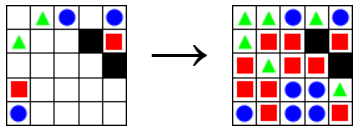
\includegraphics[scale=0.7]{img/tricky-triple.png}
    \caption{Example of Tricky Triple Puzzles, before and after solving it} \label{fig1}
\end{figure}

\section{Approach}
Throughout the development of this project, we used a Constraint Logic Programming approach.
Our grid is a list of lists, where each element is a number indicating the symbol placed on that cell.
Each one of these numbers represents a different symbol.
The number 0 represents a black cell, which cannot be generated by the solver.
The number 1 represents a green triangle,
    while the number 2 represents a red square and the number 3 a blue circle.

\subsection{Decision Variables}
All tricky triple puzzles take the form of an NxN square grid divided by cells.
The grid is represented internally by a list of lists forming a square matrix.

The grid cells can either be black, a cell that the program can't fill, or, more commonly, white.

All the white cells need to be either a triangle (represented by 1), a square (represented by 2),
    or a circle (represented by 3) to reach the puzzle solution.

The Decision Variables are all the elements of the list of lists, meaning all the puzzle cells.
Their domain is {0, 1, 2, 3}. However, being the representative of a black cell,
    the zero is not considered a valid value to fill an empty cell,
    since that would transform a white cell into a black cell.

\subsection{Constraints}
The restrictions implemented in our solver are faithful to the ones from the puzzle rules.

\textbf{Each cell must contain a symbol} \\
In the puzzle solution, all the cells have to be assigned.

\textbf{No black cells can be assigned} \\
In every white cell, we need to put a square, a triangle, or a circle.
Meaning we can't put a black cell on a white cell.

\textbf{Each group of 3 adjacent white cells (horizontally, vertically, or diagonally)
    must contain exactly 2 of one of the symbols} \\
Consider a group of three adjacent, horizontally, vertically, or diagonally, white cells.
In this group, two of the cells have the same symbol, and the last cell must have a different one.

\section{Solution Presentation}
To present the solution, we use two predicates from the file \textit{display.pl}.
\begin{itemize}
    \item The predicate \verb|display_grid/2| displays the grid in a human-friendly way so that
        the user can identify the cells and the grid's symbols.
    \item The predicate \verb|get_readable_symbol/2| translates the grid elements' internal representation
        into more readable symbols for those to be displayed to the user.
\end{itemize}

\begin{figure}
    \centering
    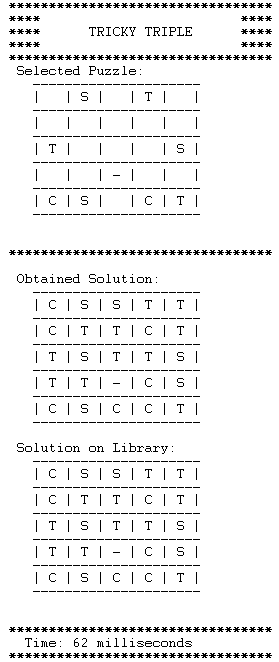
\includegraphics[scale=0.4]{img/puzzle_solving.png}
    \caption{Output Example for a Puzzle Solution} \label{fig2}
\end{figure}

\section{Experiments and Results}
The tests performed on this solver aren't as exhaustive as we could have hoped since
    we could only use the pre-generated puzzles, and there weren't that many of them.
However, we can still draw some conclusions from the times measured when solving these puzzles.

\subsection{Search Strategies}
To compensate for our lack of different puzzles, we did extensive tests with the predefined ones.
After that, we grouped the tests by the puzzle's dimension and the labeling options used in that solution.

From all the collected information, we can withdraw some conclusions:
\begin{itemize}
    \item A small board with bad labeling options can take more time to solve
            than a bigger one with good labeling options.
    \item When introducing some partially solved boards, the solver would be consistently faster.
    \item The solver's execution time increases with the increase in the grid's dimensions.
\end{itemize}

The graph below illustrates the obtained results.
Table \ref{tab1} contains the average values for each dimension and labeling option.

\begin{figure}
    \centering
    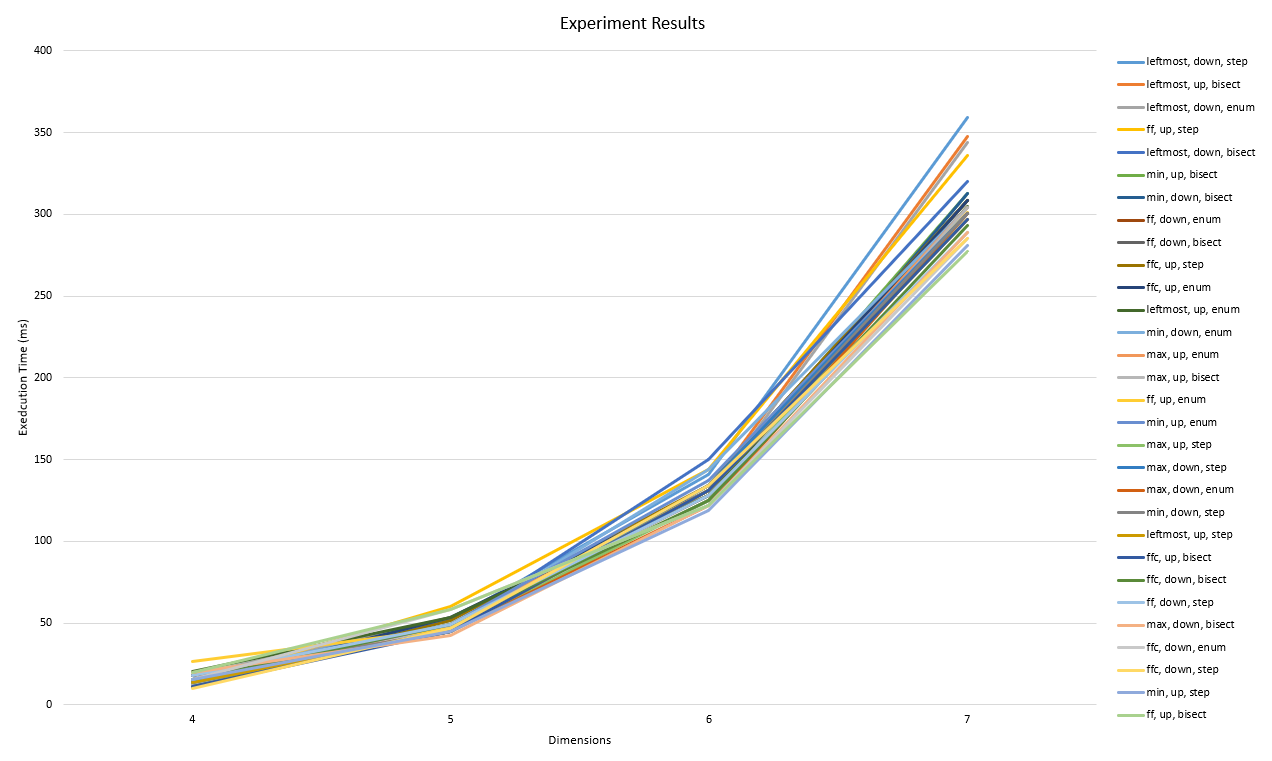
\includegraphics[width=\textwidth]{img/execution_times.png}
    \caption{Experiment Results} \label{fig3}
\end{figure}
Analyzing Figure \ref{fig3}, we can conclude that the fastest labeling option,
    for grids up to 7x7, is "ff, up, bisect".

However, using the same data, we can try to predict the behavior of the labeling options
    when increasing the grid's dimensions by making a trendline.
Using a degree 3 polynomial trendline, we obtained a prediction for execution times when solving bigger grids.
The equations for these trendlines are in Table \ref{tab2}.
Analyzing Figure \ref{fig4}, we can conclude that perhaps the best options would be
    "min, down, enum" or "leftmost, down, bisect".

\begin{figure}
    \centering
    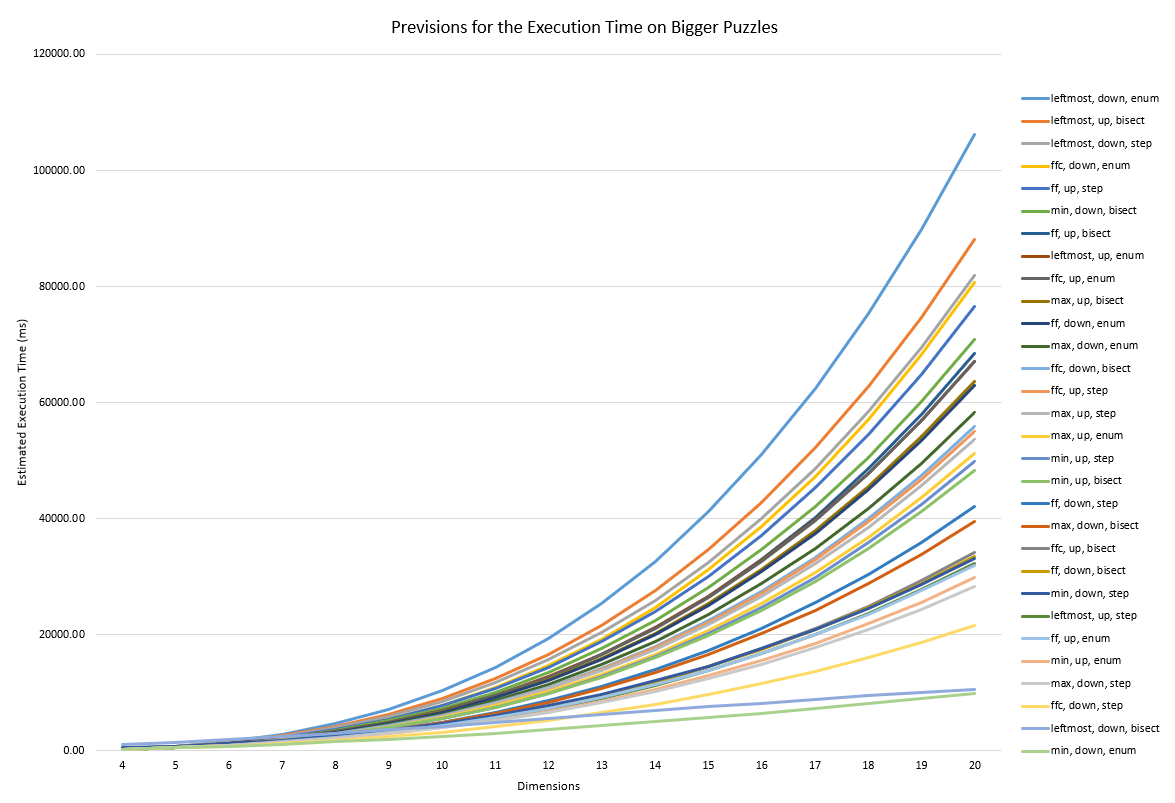
\includegraphics[width=\textwidth]{img/previsions.png}
    \caption{Execution Times Predictions} \label{fig4}
\end{figure}

\subsection{Dimensional Analysis}

\section{Conclusions and Future Work}

\section{Bibliography}

\section{Annex}

\subsection{Average Execution Times Table} \label{experiment-results}

\begin{table}
    \caption{Average Times Obtained (ms)} \label{tab1}
    \begin{tabularx}{\textwidth}{|C|C|C|C|C|C|C|}
        \hline
        \multicolumn{3}{|c|}{Labeling} & \multicolumn{4}{|c|}{Grids} \\
        \cline{4-7}
        \multicolumn{3}{|c|}{Options} & 4x4 & 5x5 & 6x6 & 7x7 \\
        \hline
        leftmost & up   & step   & 13.43 & 44.57 & 131.4  & 296.75 \\
        leftmost & up   & enum   & 20.14 & 53.57 & 128    & 304.75 \\
        leftmost & up   & bisect & 13.43 & 46.86 & 131.2  & 347.75 \\
        leftmost & down & step   & 17.71 & 51.43 & 140.6  & 359.25 \\
        leftmost & down & enum   & 17.86 & 53.57 & 128.2  & 343.75 \\
        leftmost & down & bisect & 17.71 & 47    & 150    & 320.25 \\
        ff       & up   & step   & 13.42 & 60.14 & 143.8  & 336    \\
        ff       & up   & enum   & 26.71 & 46.86 & 131.2  & 301    \\
        ff       & up   & bisect & 20    & 58    & 122    & 277.25 \\
        ff       & down & step   & 18    & 49.14 & 128    & 289    \\
        ff       & down & enum   & 15.71 & 49.14 & 128    & 308.5  \\
        ff       & down & bisect & 15.71 & 44.57 & 134.4  & 308.5  \\
        ffc      & up   & step   & 11.14 & 51.43 & 134.4  & 308.5  \\
        ffc      & up   & enum   & 13.29 & 53.57 & 131.4  & 308.5  \\
        ffc      & up   & bisect & 11.14 & 44.57 & 131.4  & 296.75 \\
        ffc      & down & step   &  9.71 & 46.86 & 134.4  & 285    \\
        ffc      & down & enum   & 15.57 & 58.14 & 121.8  & 285.25 \\
        ffc      & down & bisect & 15.57 & 49    & 125    & 293    \\
        min      & up   & step   & 15.71 & 44.58 & 118.8  & 281.25 \\
        min      & up   & enum   & 15.57 & 49.14 & 137.4  & 300.75 \\
        min      & up   & bisect & 13.43 & 44.71 & 131.2  & 312.5  \\
        min      & down & step   & 17.86 & 44.57 & 131.4  & 300.5  \\
        min      & down & enum   & 15.71 & 46.86 & 143.8  & 304.5  \\
        min      & down & bisect & 13.43 & 46.86 & 125    & 312.5  \\
        max      & up   & step   & 13.43 & 44.58 & 125    & 300.75 \\
        max      & up   & enum   & 13.43 & 49    & 131.4  & 304.5  \\
        max      & up   & bisect & 13.29 & 47    & 125    & 304.5  \\
        max      & down & step   & 13.43 & 44.71 & 134.4  & 300.75 \\
        max      & down & enum   & 17.86 & 44.58 & 122    & 300.75 \\
        max      & down & bisect & 20    & 42.43 & 122    & 289    \\
        \hline
    \end{tabularx}
\end{table}

\subsection{Trendlines using to Estimate Execution Time for Bigger Grids} \label{trendlines}

\begin{table}
    \caption{Trendlines} \label{tab2}
    \begin{tabularx}{\textwidth}{|C|C|C|C|C|}
        \hline
        \multicolumn{3}{|c|}{Labeling Options} & \multicolumn{2}{|c|}{Equations} \\
        \hline
        leftmost & up   & step   & \multicolumn{2}{|c|}{\(y = ax^3 + bx^2 + cx + d = 0 \)} \\
        leftmost & up   & enum   & \multicolumn{2}{|c|}{\(y = ax^3 + bx^2 + cx + d = 0 \)} \\
        leftmost & up   & bisect & \multicolumn{2}{|c|}{\(y = ax^3 + bx^2 + cx + d = 0 \)} \\
        leftmost & down & step   & \multicolumn{2}{|c|}{\(y = ax^3 + bx^2 + cx + d = 0 \)} \\
        leftmost & down & enum   & \multicolumn{2}{|c|}{\(y = ax^3 + bx^2 + cx + d = 0 \)} \\
        leftmost & down & bisect & \multicolumn{2}{|c|}{\(y = ax^3 + bx^2 + cx + d = 0 \)} \\
        ff       & up   & step   & \multicolumn{2}{|c|}{\(y = ax^3 + bx^2 + cx + d = 0 \)} \\
        ff       & up   & enum   & \multicolumn{2}{|c|}{\(y = ax^3 + bx^2 + cx + d = 0 \)} \\
        ff       & up   & bisect & \multicolumn{2}{|c|}{\(y = ax^3 + bx^2 + cx + d = 0 \)} \\
        ff       & down & step   & \multicolumn{2}{|c|}{\(y = ax^3 + bx^2 + cx + d = 0 \)} \\
        ff       & down & enum   & \multicolumn{2}{|c|}{\(y = ax^3 + bx^2 + cx + d = 0 \)} \\
        ff       & down & bisect & \multicolumn{2}{|c|}{\(y = ax^3 + bx^2 + cx + d = 0 \)} \\
        ffc      & up   & step   & \multicolumn{2}{|c|}{\(y = ax^3 + bx^2 + cx + d = 0 \)} \\
        ffc      & up   & enum   & \multicolumn{2}{|c|}{\(y = ax^3 + bx^2 + cx + d = 0 \)} \\
        ffc      & up   & bisect & \multicolumn{2}{|c|}{\(y = ax^3 + bx^2 + cx + d = 0 \)} \\
        ffc      & down & step   & \multicolumn{2}{|c|}{\(y = ax^3 + bx^2 + cx + d = 0 \)} \\
        ffc      & down & enum   & \multicolumn{2}{|c|}{\(y = ax^3 + bx^2 + cx + d = 0 \)} \\
        ffc      & down & bisect & \multicolumn{2}{|c|}{\(y = ax^3 + bx^2 + cx + d = 0 \)} \\
        min      & up   & step   & \multicolumn{2}{|c|}{\(y = ax^3 + bx^2 + cx + d = 0 \)} \\
        min      & up   & enum   & \multicolumn{2}{|c|}{\(y = ax^3 + bx^2 + cx + d = 0 \)} \\
        min      & up   & bisect & \multicolumn{2}{|c|}{\(y = ax^3 + bx^2 + cx + d = 0 \)} \\
        min      & down & step   & \multicolumn{2}{|c|}{\(y = ax^3 + bx^2 + cx + d = 0 \)} \\
        min      & down & enum   & \multicolumn{2}{|c|}{\(y = ax^3 + bx^2 + cx + d = 0 \)} \\
        min      & down & bisect & \multicolumn{2}{|c|}{\(y = ax^3 + bx^2 + cx + d = 0 \)} \\
        max      & up   & step   & \multicolumn{2}{|c|}{\(y = ax^3 + bx^2 + cx + d = 0 \)} \\
        max      & up   & enum   & \multicolumn{2}{|c|}{\(y = ax^3 + bx^2 + cx + d = 0 \)} \\
        max      & up   & bisect & \multicolumn{2}{|c|}{\(y = ax^3 + bx^2 + cx + d = 0 \)} \\
        max      & down & step   & \multicolumn{2}{|c|}{\(y = ax^3 + bx^2 + cx + d = 0 \)} \\
        max      & down & enum   & \multicolumn{2}{|c|}{\(y = ax^3 + bx^2 + cx + d = 0 \)} \\
        max      & down & bisect & \multicolumn{2}{|c|}{\(y = ax^3 + bx^2 + cx + d = 0 \)} \\
        \hline
    \end{tabularx}
\end{table}

%%%%%%%%%%%%%%%%%%%%%%%%%%%%%%%%%%%%%%%%%%%%%%%%%%%%%%%%%%%%%%%%%%%%%%%%%%%%%%%%%%%

\section{Section Sample}
\subsection{A Subsection Sample}
Please note that the first paragraph of a section or subsection is
not indented. The first paragraph that follows a table, figure,
equation etc. does not need an indent, either.

Subsequent paragraphs, however, are indented.

\subsubsection{Sample Heading (Third Level)} Only two levels of
headings should be numbered. Lower level headings remain unnumbered;
they are formatted as run-in headings.

\paragraph{Sample Heading (Fourth Level)}
The contribution should contain no more than four levels of
headings. Table~\ref{tab1} gives a summary of all heading levels.

\begin{table}
\caption{Table captions should be placed above the
tables.}\label{example_table}
\begin{tabular}{|l|l|l|}
\hline
Heading level &  Example & Font size and style\\
\hline
Title (centered) &  {\Large\bfseries Lecture Notes} & 14 point, bold\\
1st-level heading &  {\large\bfseries 1 Introduction} & 12 point, bold\\
2nd-level heading & {\bfseries 2.1 Printing Area} & 10 point, bold\\
3rd-level heading & {\bfseries Run-in Heading in Bold.} Text follows & 10 point, bold\\
4th-level heading & {\itshape Lowest Level Heading.} Text follows & 10 point, italic\\
\hline
\end{tabular}
\end{table}


\noindent Displayed equations are centered and set on a separate
line.
\begin{equation}
x + y = z
\end{equation}

Please try to avoid rasterized images for line-art diagrams and
schemas. Whenever possible, use vector graphics instead (see
Fig.~\ref{fig1}).

\begin{figure}

\includegraphics[width=\textwidth]{img/FEUPlogo.png}
\caption{A figure caption is always placed below the illustration.
Please note that short captions are centered, while long ones are
justified by the macro package automatically.} \label{fig_example}
\end{figure}

\begin{theorem}
This is a sample theorem. The run-in heading is set in bold, while
the following text appears in italics. Definitions, lemmas,
propositions, and corollaries are styled the same way.
\end{theorem}
%
% the environments 'definition', 'lemma', 'proposition', 'corollary',
% 'remark', and 'example' are defined in the LLNCS documentclass as well.
%
\begin{proof}
Proofs, examples, and remarks have the initial word in italics,
while the following text appears in normal font.
\end{proof}
For citations of references, we prefer the use of square brackets
and consecutive numbers. Citations using labels or the author/year
convention are also acceptable. The following bibliography provides
a sample reference list with entries for journal
% TODO
%articles~\cite{ref_article1}, an LNCS chapter~\cite{ref_lncs1}, a
%book~\cite{ref_book1}, proceedings without editors~\cite{ref_proc1},
%and a homepage~\cite{ref_url1}. Multiple citations are grouped
%\cite{ref_article1,ref_lncs1,ref_book1},
%\cite{ref_article1,ref_book1,ref_proc1,ref_url1}.
%
% ---- Bibliography ----
%
% BibTeX users should specify bibliography style 'splncs04'.
% References will then be sorted and formatted in the correct style.
%
% \bibliographystyle{splncs04}
% \bibliography{mybibliography}
%
\begin{thebibliography}{8}
\bibitem{ref_article1}
Author, F.: Article title. Journal \textbf{2}(5), 99--110 (2016)

\bibitem{ref_lncs1}
Author, F., Author, S.: Title of a proceedings paper. In: Editor,
F., Editor, S. (eds.) CONFERENCE 2016, LNCS, vol. 9999, pp. 1--13.
Springer, Heidelberg (2016). \doi{10.10007/1234567890}

\bibitem{ref_book1}
Author, F., Author, S., Author, T.: Book title. 2nd edn. Publisher,
Location (1999)

\bibitem{ref_proc1}
Author, A.-B.: Contribution title. In: 9th International Proceedings
on Proceedings, pp. 1--2. Publisher, Location (2010)

\bibitem{ref_url1}
LNCS Homepage, \url{http://www.springer.com/lncs}. Last accessed 4
Oct 2017
\end{thebibliography}

\end{document}
